\documentclass[11pt]{amsart}
\usepackage{geometry}                % See geometry.pdf to learn the layout options. There are lots.
\geometry{letterpaper}                   % ... or a4paper or a5paper or ... 
%\geometry{landscape}                % Activate for for rotated page geometry
%\usepackage[parfill]{parskip}    % Activate to begin paragraphs with an empty line rather than an indent
\usepackage{graphicx}
\usepackage{amssymb}
\usepackage{epstopdf}
\DeclareGraphicsRule{.tif}{png}{.png}{`convert #1 `dirname #1`/`basename #1 .tif`.png}

\raggedbottom

 
\begin{document}
 
 \title{Biological analogues for $ V $-variable fractals}  
\author{John E.\ Hutchinson}
\date{\today}
 
 
 \maketitle
 
 No new mathematics here!
 
\bigskip  

% 
% 
%\bigskip 
%\begin{center} 
%   
\includegraphics[width=2cm]{SG2,3.jpg} 
%\end{center}


\section{Background}
The \emph{ergodic point process} (\emph{forward process} or \emph{chaos game}) for $ SG(2) $  consists of selecting a starting point $ x_0 $ and a sequence of maps $ (g_i)_{i\geq 1} $ from $ F=\{g_1,g_2,g_3  \} $ in an iid manner according to some fixed probability distribution $ P $.  Then the sequence of points
\[
x_0,\  x_1=g_1(x_0),\  x_2 = g_2\circ g_1(x_0), \  g_3\circ g_2 \circ g_0 (x_0),                   \dots ,
\]
converges a.s.\  to $  SG(2) $.       
More precisely, the sequence of unit measures
\[
\frac{1}{n} \big(\delta_{x_0}+\cdots + \delta_{x_{n-1}}\big)
\]
converges in the weak sense of measures to the natural measure on $ SG(2) $ induced from $ P $.

\bigskip
The \emph{convergent point process} (\emph{backward process}) takes many sequences of the form:
\[
x_0,  \  x_1 = g_1(x_0),\  x_2 = g_1\circ g_2(x_0),\  x_3 = g_1\circ g_2 \circ g_3 (x_0), \dots 
\]
Note the order of composition.  Each sequence will converge to a point on $ SG(2) $.  Running the process many times gives a sample of points on $ SG(2) $ whose empirical distribution converges a.s.\ to the natural distribution on $ SG(2) $ given by $ P $.


\bigskip
The \emph{convergent set process}, a convergent sequence of approximating compact sets, says that for any initial non empty compact $ K $, the sequence of sets
\[
K, F(K), F^{\circ 2}(K), F^{\circ 3}(K), \dots \to SG(2),\]
in the Hausdorff  sense, where 
\[ F(E) := f_1(E) \cup f_2(E) \cup f_3(E). \]






%%%%%%%%%%%%%%%%%%%%%%%%%%%%%%%%%%%%%%%%%%%%%%%%%
%%%%%%%%%%%%%%%%%%%%%%%%%%%%%%%%%%%%%%%%%%%%%%%%%
%%%%%%%%%%%%%%%%%%%%%%%%%%%%%%%%%%%%%%%%%%%%%%%%%
\section{Convergent Process for Generating $ V $-Variable Fractals} This is the analogue of the convergent point process for a deterministic fractal.   The analogue of a point is a $ V $-tuple of compact sets, the analogue of the deterministic fractal is a superfractal, and the analogue of a point on the deterministic fractal is a $ V $-variable $ V $-tuple of fractals (which will be the elements of the superfractal).
 
 
\medskip  Here we grow organisms from an initial cell (or cells). The transformations rules are interpreted as \emph{replacement/division}   rules. 

Later we grow trees, and the transformation rules are interpreted as branching behaviour at the buds of the previous generation tree.
   
\bigskip Consider the case $ V=4 $. 

The bottom line of Figure~\ref{bp} shows the four possible types for the initial cell.  The   division rules at time 1 are shown next and  are followed by the 4 resulting organisms at time 1.  The transformation rules at time 2 are then followed by the resulting organisms at time 2.  Finally, the transformation rules at time 3 are followed by the resulting organisms at time~3. 
   
   Note that the 4 organisms/embryos do not interact and in that sense grow  independently on one another, in a manner determined only by the choice of transformations at each time.   This is distinct from the situation for the forward process, as we see in Section~\ref{forp}.   For this reason the backward process could probably be  best understood by just following the development from one cell, as in Figure~\ref{bp1}. 
   
   
\medskip     The choice of transformation rules could be an iid or Markovian process, for example. 

\medskip Next observe any of the four  growing organisms at successive times and ignore the cell type, i.e.\ colour. 
 The organism structure at each time is a refinement  of the organism at the previous time.  This is more easily seen in Figure~\ref{V-vargenblack}, where colours are suppressed and the development beginning from the green cell is shown. It is \emph{important} however, to note that in order to actually construct the sequence, the colour information, that is the type of each cell, is needed in order to pass from one level to the next.
 
 The colours are a way of keeping track of the cell type at each level.  In the $ V $-variable case there are at most $ V $-types at each level.
  
 \bigskip
 In standard terminology, Figure~\ref{bp} is described as follows:
  \begin{enumerate}
\item The first (bottom) row denotes a   4-tuple of sets $ \boldsymbol{K^0}= (\boldsymbol{K^0}_1,\dots, \boldsymbol{K^0}_4) $  =  (Red, Green, Yellow, Black).
  \item The second row denotes the operator $ \boldsymbol{\Phi}^{a_1} $  and the third row denotes 
  $\boldsymbol{K^1} =   \boldsymbol{\Phi}^{a_1} ( \boldsymbol{K^0}) $.
  \item The fourth row denotes  $ \boldsymbol{\Phi}^{a_2} $  and the fifth  row denotes 
  $\boldsymbol{K^2} =   \boldsymbol{\Phi}^{a_1}\circ \boldsymbol{\Phi}^{a_2}  ( \boldsymbol{K^0}) $.
  \item The sixth row denotes  $ \boldsymbol{\Phi}^{a_3} $  and the seventh  row denotes 
  $\boldsymbol{K^3} =   \boldsymbol{\Phi}^{a_1} \circ  \boldsymbol{\Phi}^{a_2}\circ \boldsymbol{\Phi}^{a_3}  ( \boldsymbol{K^0}) $.
  \end{enumerate} 
 
 Note that the sequence 
\[ \boldsymbol{K^0}, \boldsymbol{K^1}, \boldsymbol{K^2}, \boldsymbol{K^3}, \dots \]
converges to a \emph{single} 4-variable 4-tuple of sets.

\medskip  Again using standard terminology, the sequence in Figure~\ref{bp1} is 
\[  \boldsymbol{K^0}_2,  \boldsymbol{K^1}_2, \boldsymbol{K^2}_2, \boldsymbol{K^3}_2, \dots \]
 
 
\begin{figure}[htbp] %  figure placement: here, top, bottom, or page
   \centering
   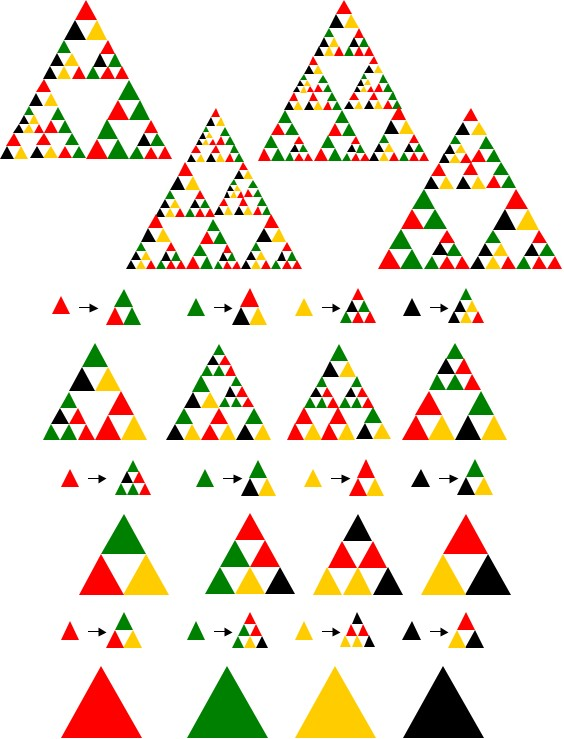
\includegraphics[width=5in]{V-vargenA.jpg} 
    \caption{\textbf{Backward (actually Retarded) Process.} Organism growth from  initial cells.  Transformations rules interpreted as \emph{replacement/division}   rules.}
   \label{bp}
   \end{figure}
   
   \begin{figure}[htbp] %  figure placement: here, top, bottom, or page
   \centering
   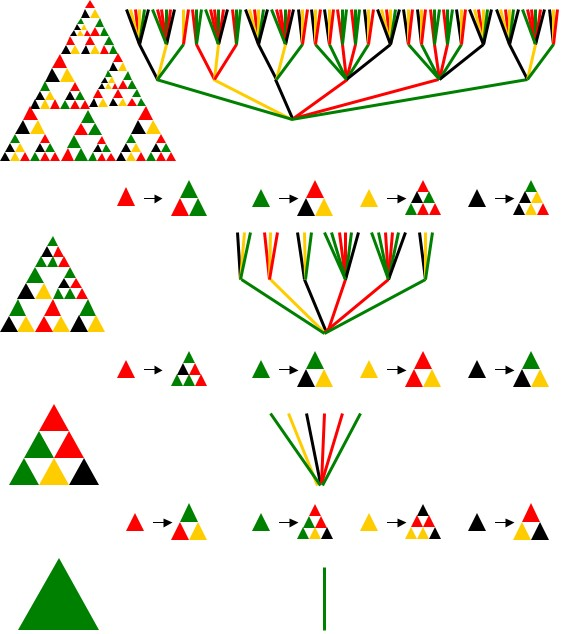
\includegraphics[width=5in]{V-vargenA1.jpg} 
   \caption{\textbf{Convergent Process.} Embryo/Organism growth from  an initial green cell only.  Same rules as in Figure~\ref{bp}.   Shown in the left column, from the bottom up, are $ \boldsymbol{K^0}_2 $, \qquad 
$\boldsymbol{K^1}_2 =  \big( \boldsymbol{\Phi}^{a_1} ( \boldsymbol{K^0})\big)_2 $,    \qquad 
 $\boldsymbol{K^2}_2 =   \big(\boldsymbol{\Phi}^{a_1}\circ \boldsymbol{\Phi}^{a_2}  ( \boldsymbol{K^0})\big)_2 $,    $\boldsymbol{K^3}_2 =   \big(\boldsymbol{\Phi}^{a_1} \circ  \boldsymbol{\Phi}^{a_2}\circ \boldsymbol{\Phi}^{a_3}  ( \boldsymbol{K^0})\big)_2 $.
   \quad    Alternatively, the analogous tree growth from an initial green limb, with 4 types of limbs in general and associated branching determined by the $\boldsymbol{\Phi}^{a} $, is also shown.  Note that the tree diagram encodes the complete construction information, unlike the embryo diagram. The top tree here is the bottom tree in Figure~\ref{treeg}. 
}
   \label{bp1}
   \end{figure}
  
 \mbox{} \bigskip \mbox{}
   
\begin{figure}[htbp] %  figure placement: here, top, bottom, or page
   \centering
   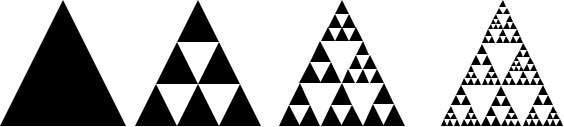
\includegraphics[width=5in]{V-vargenblack.jpg} \quad 
   \caption{Organism development via cell division.  Each embryo is a refinement of the embryo at the previous time.
   Same as growth from green cell, with colours suppressed here.
   \vspace{1cm}}
   \label{V-vargenblack}
\end{figure}
 
   
\begin{figure}[htbp] %  figure placement: here, top, bottom, or page
   \centering
   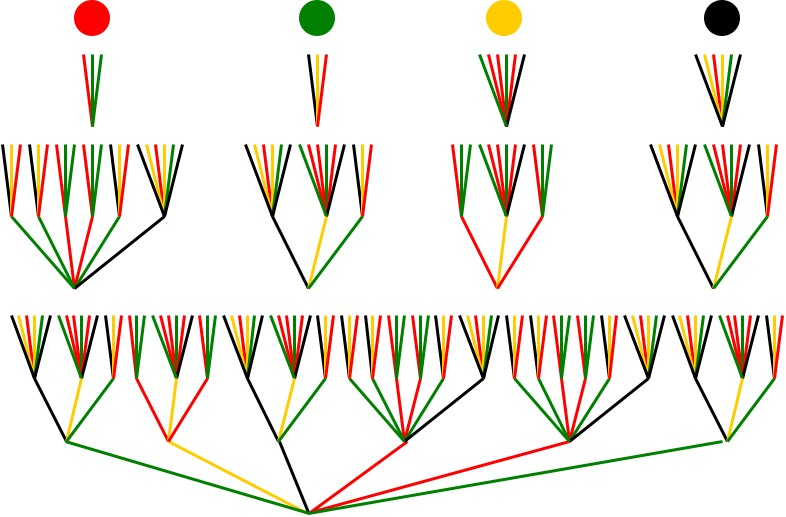
\includegraphics[width=5in]{limseq.jpg} \quad 
   \caption{The dots at the top show the colours representing the 4 components.
   The top row of trees is   $ \boldsymbol{\Phi}^{a_3} ( \boldsymbol{K^0}) $.  The next row is 
 $    \boldsymbol{\Phi}^{a_2}\circ \boldsymbol{\Phi}^{a_3}  ( \boldsymbol{K^0}) $.  The bottom row
    is $  \boldsymbol{\Phi}^{a_1} \circ  \boldsymbol{\Phi}^{a_2}\circ \boldsymbol{\Phi}^{a_3}  ( \boldsymbol{K^0}) $, with just the second component showing. Compare with Figure~\ref{bp1}, which gives  bottom up tree growth, whereas here we have top down tree development/description.}
   \label{treeg}
\end{figure}
 


%\begin{figure}[htbp] %  figure placement: here, top, bottom, or page
%   \centering
%   
\includegraphics[width=1in]{V-vargenblack0.jpg} \quad 
%   
\includegraphics[width=1in]{V-vargenblack1.jpg} \quad  
%   
\includegraphics[width=1in]{V-vargenblack2.jpg} \quad 
%   
\includegraphics[width=1in]{V-vargenblack3.jpg} 
%   \caption{Organism development via cell division.  Each embryo is a refinement of the embryo at the previous time.
%   Same as growth from green cell, with colours suppressed here.}
%   \label{V-vargenblack}
%\end{figure}
% 



%%%%%%%%%%%%%%%%%%%%%%%%%%%%%%%%%%%%%%%%%%%%%%%%%
%%%%%%%%%%%%%%%%%%%%%%%%%%%%%%%%%%%%%%%%%%%%%%%%%
%%%%%%%%%%%%%%%%%%%%%%%%%%%%%%%%%%%%%%%%%%%%%%%%%
\clearpage \section{Backward Process for Generating $ V $-Variable Trees}

Here we interpret the transformation rules as growth rules at the top of each limb.

\begin{figure}[htbp] %  figure placement: here, top, bottom, or page
   \centering
   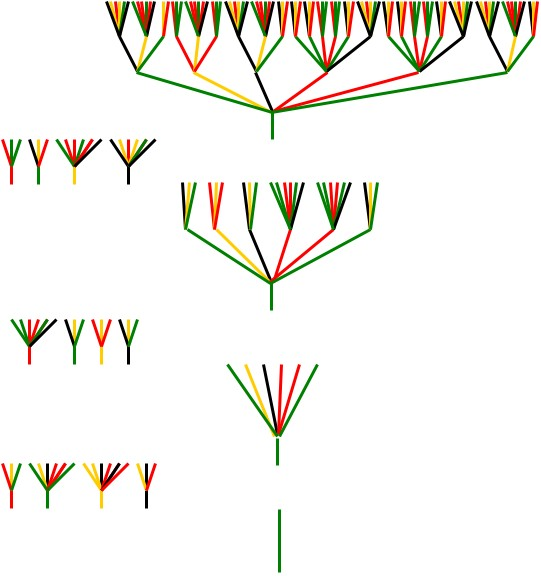
\includegraphics[width=5in]{V-tree.jpg} \quad 
   \caption{Tree growth.  Each limb is one of $ V=4 $ types.  The transformation rules at each stage determine how a particular type of limb grows.  Here we begin with a single green type limb.  The rules here are the same as in Figure~\ref{bp}.}
   \label{treegr}
\end{figure}




%%%%%%%%%%%%%%%%%%%%%%%%%%%%%%%%%%%%%%%%%%%%%%%%%
%%%%%%%%%%%%%%%%%%%%%%%%%%%%%%%%%%%%%%%%%%%%%%%%%
%%%%%%%%%%%%%%%%%%%%%%%%%%%%%%%%%%%%%%%%%%%%%%%%%


\clearpage \section{Forward Process for Generating $ V $-Variable Fractals} \label{forp}
 

 Here we breed organisms from other organisms.  The transformations rules are interpreted as \emph{combination}   rules.  The selected rules are the same as before, but interpreted differently.
 
  Begin with one individual organism of each of 4 types, ignoring any fine detail.  The first set of combination rules produce 4 new organisms, one  of each type.  The second set produces another 4 and the third set produces another 4.  After a few initial iterations, successive iterations produce a collection of organisms, 4 for each iteration, whose empirical distribution converges to the theoretical distribution of $ V $-variable fractals.
  

\medskip   The selected rules are the same as for the backward algorithm, but are applied differently.

\medskip   If the transformations rules are selected by the same stochastic process in each case then the probability distribution on organisms is the same.  

In the backward case \emph{one} run of the experiment gives \emph{one} four tuple of organisms.  Running the experiment \emph{many} times provides an empirical approximation to the induced probability distribution on organisms.

In the forward case, \emph{one} run of the experiment ergodically samples the full distribution of 4-tuples of individuals.

\medskip 
 In standard terminology:
  \begin{enumerate}
\item The first (bottom) row denotes a   4-tuple of sets $ \boldsymbol{K^0}= (K_1,\dots, K_4) $.
  \item The second row denotes the operator $ \boldsymbol{\Phi}^{a_1} $  and the third row denotes 
  $\boldsymbol{K^1} =   \boldsymbol{\Phi}^{a_1} (K^0) $.
  \item The fourth row denotes  $ \boldsymbol{\Phi}^{a_2} $  and the fifth  row denotes 
  $\boldsymbol{K^2} =    \boldsymbol{\Phi}^{a_2}  (K^1) $.
  \item The sixth row denotes  $ \boldsymbol{\Phi}^{a_3} $  and the seventh  row denotes 
  $\boldsymbol{K^3} =   \boldsymbol{\Phi}^{a_3}   (K^2) $.
  \end{enumerate} 
 
 Note that the sequence 
\[ \boldsymbol{K^0}, \boldsymbol{K^1}, \boldsymbol{K^2}, \boldsymbol{K^3}, \dots \]
moves \emph{ergodically through} the set of   4-variable 4-tuple of sets.
 
  \begin{figure}[htbp] %  figure placement: here, top, bottom, or page
   \centering
   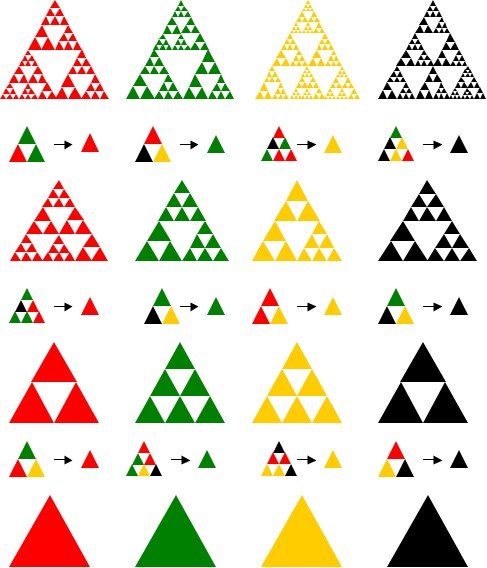
\includegraphics[width=4in]{V-vargenB.jpg} 
   \caption{\textbf{Forward Process.} Transformations rules interpreted as \emph{combination}   rules.}
      \label{V-vargenB}
\end{figure}
 
 
 %%%%%%%%%%%%%%%%%%%%%%%%%%%%%%%%%%%%%%%%%%%%%%%%%
%%%%%%%%%%%%%%%%%%%%%%%%%%%%%%%%%%%%%%%%%%%%%%%%%
%%%%%%%%%%%%%%%%%%%%%%%%%%%%%%%%%%%%%%%%%%%%%%%%%


\clearpage \section{Forward Process for Generating $ V $-Variable Trees} \label{forp}

A $ V $-tuple of labelled trees is generated at each step, from a $ V $-tuple of labelled trees at the previous step, by means of 
 transformation rules.  In Figure~\ref{V-treef} we have two IFSs, one for $ SG(2) $ and one for $ SG(3) $.  Since the branching number determines the IFS in this case, we do not explicitly show the IFS.
 
Starting from the bottom, the 4 transformation rules at the   left determine the initial 4 subtrees and the type (colour) of each limb (or edge).
The coloured dot at the bottom of the tree gives the ``type'' of the tree.

The next four transformation rules   give 4 new subtrees, and the colour  of a limb  tell us which of the 4 previous subtrees should be attached to the top of the limb.

The next four   transformation rules   again give 4 new subtrees, and the colour  of a limb  again tell us which of the 4 previous subtrees should be attached to the top of the limb.

Etc.
 
Each limb is one of 4 possible types, and the subtree rooted at the top of the limb can also be regarded as of the same type.

  \begin{figure}[htbp] %  figure placement: here, top, bottom, or page
   \centering
   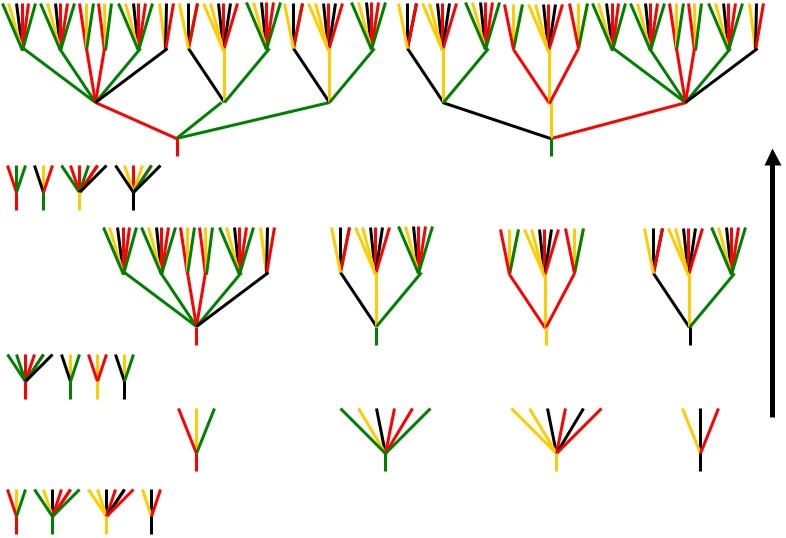
\includegraphics[width=6in]{V-treef.jpg} 
   \caption{\textbf{Forward Process.} Transformations rules interpreted as \emph{combination}   rules.}
      \label{V-treef}
\end{figure}


 
%%%%%%%%%%%%%%%%%%%%%%%%%%%%%%%%%%%%%%%%%%%%%%%%%
%%%%%%%%%%%%%%%%%%%%%%%%%%%%%%%%%%%%%%%%%%%%%%%%%
%%%%%%%%%%%%%%%%%%%%%%%%%%%%%%%%%%%%%%%%%%%%%%%%%
\clearpage \section{Necks} \label{secneck}
 
\begin{figure}[htbp] %  figure placement: here, top, bottom, or page
   \centering
   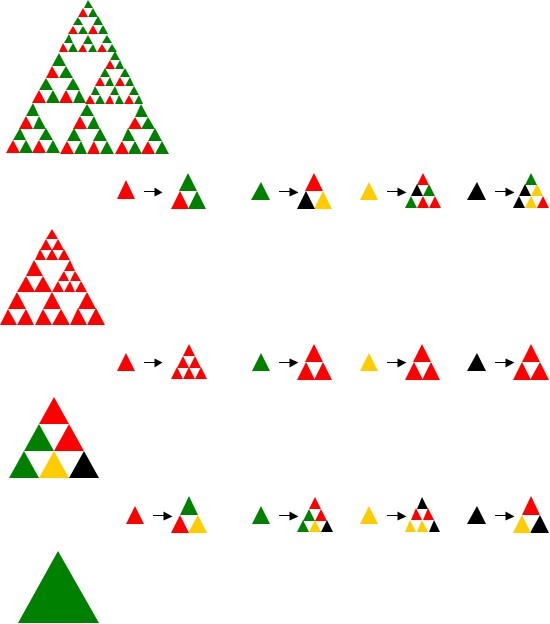
\includegraphics[width=5in]{V-vargenAn.jpg} 
   \caption{\textbf{Backward (actually Retarded) Process.} Organism growth from  initial green cell.  
$  \boldsymbol{\Phi}^{a_2}    $ is a neck.}
   \label{neck}
   \end{figure}







%%%%%%%%%%%%%%%%%%%%%%%%%%%%%%%%%%%%%%%%%%%%%%%%%
%%%%%%%%%%%%%%%%%%%%%%%%%%%%%%%%%%%%%%%%%%%%%%%%%
%%%%%%%%%%%%%%%%%%%%%%%%%%%%%%%%%%%%%%%%%%%%%%%%%

\newpage \section{Superfractal} \label{secsf}
 The previously described forward process for $ V $-variable fractals is the forward process on the superfractal attractor.   The backward process is really  the retarded process on the superfractal attractor. 
 
\begin{figure}[htbp] 
\centering
   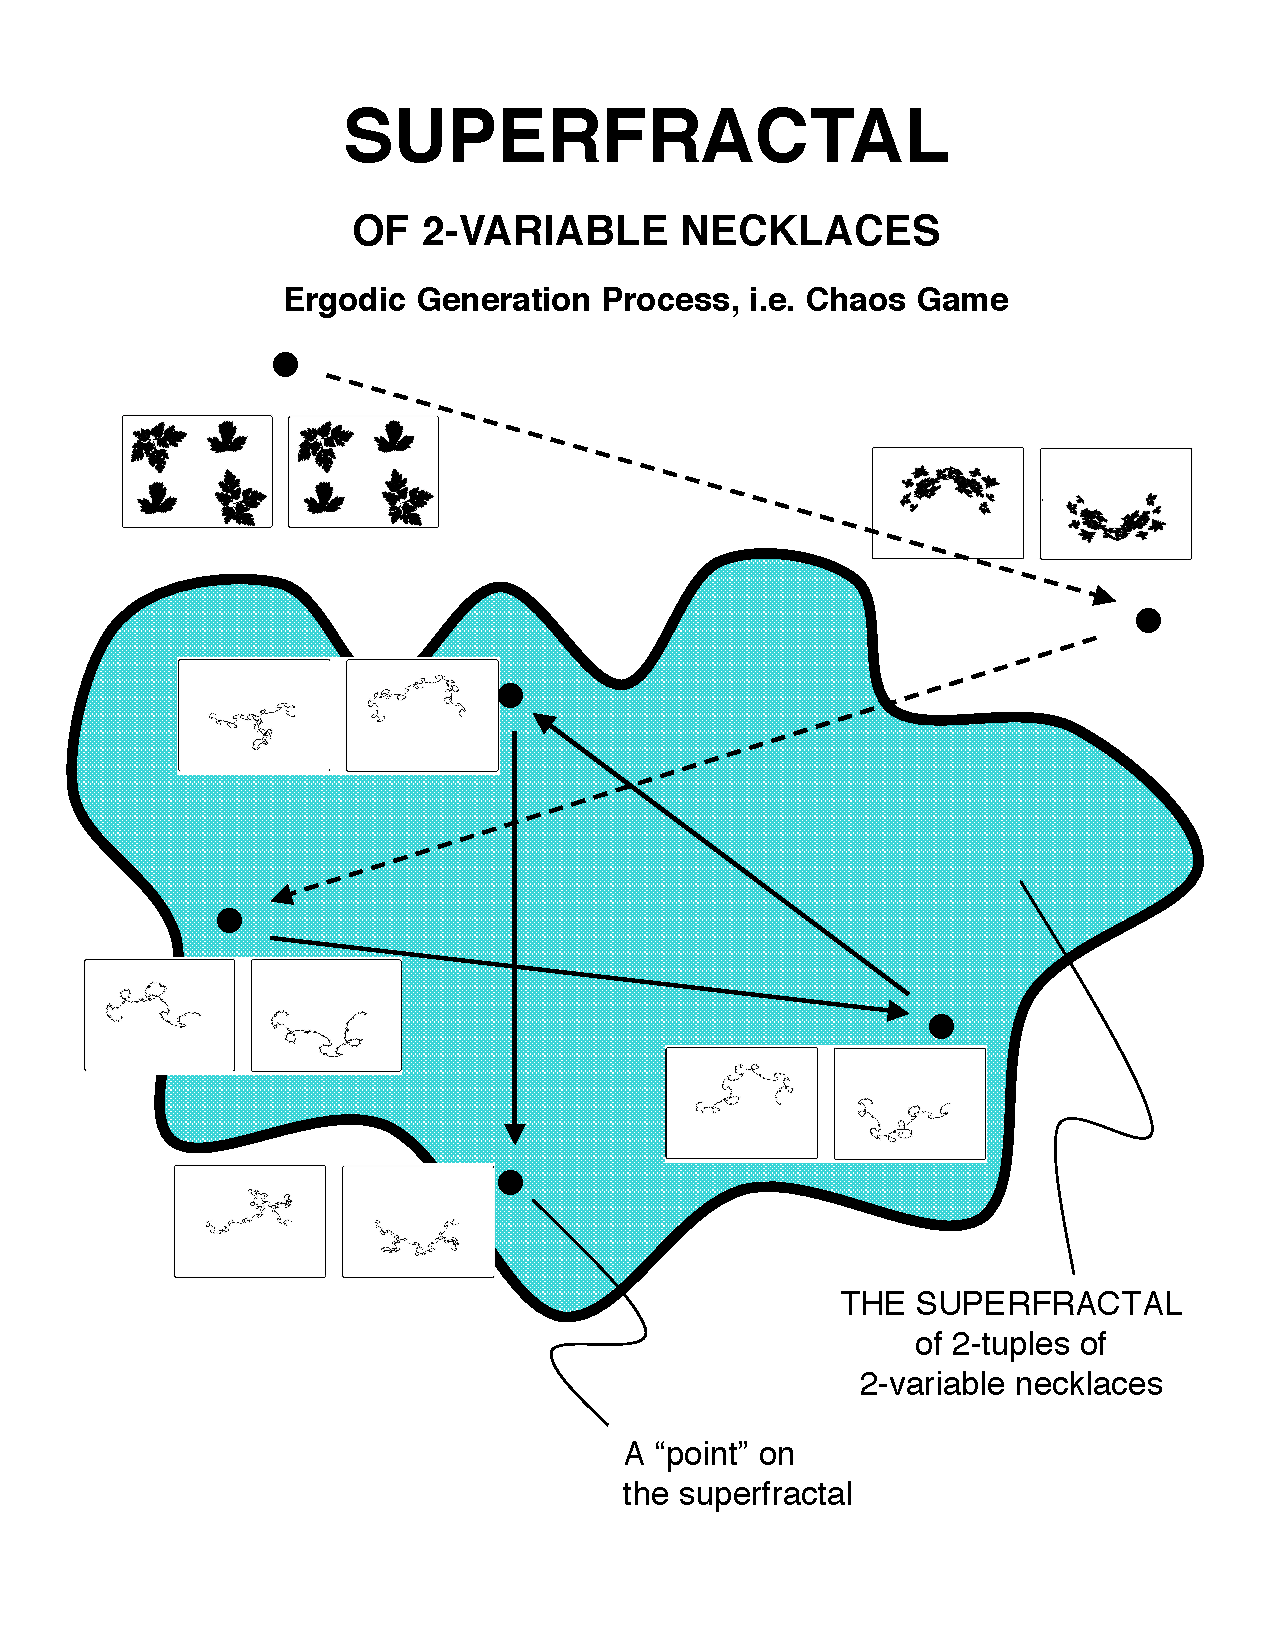
\includegraphics[width=4in]{Superfractal.pdf} 
   \caption{Superfractal}
\end{figure}

 
 
 
 
 
 
 
 
 
 
 
 
 
 \end{document}  